%----------------------------------------------------------------------------------------
%	PACKAGES AND OTHER DOCUMENT CONFIGURATIONS
%----------------------------------------------------------------------------------------

\documentclass[sigconf]{acmart}

\usepackage[english]{babel}

\settopmatter{printacmref=false}
\renewcommand\footnotetextcopyrightpermission[1]{}
\pagestyle{plain}

\usepackage{titlesec} % Allows customization of titles
\titleformat{\section}[block]{\large\scshape\leftalign}{\thesection.}{1em}{}
\titleformat{\subsection}[block]{\large}{\thesubsection.}{1em}{}

\usepackage{hyperref}

%----------------------------------------------------------------------------------------
%	TITLE & AUTHORS SECTION
%----------------------------------------------------------------------------------------

\begin{document}

\title{Recognizing emotions with technology and starting discussions}
\subtitle{Research in Emerging Technologies 2017-2018, final paper}
\date{January 2018}

\author{Randall Theuns}
\affiliation{%
    \institution{Amsterdam University of Applied Sciences}
    \department{Software Engineering}
    \streetaddress{Wibautstraat 2-4}
    \city{Amsterdam}
    \postcode{1091GM}
    \country{The Netherlands}
}
\email{randall.theuns@hva.nl}

\author{Max Beije}
\affiliation{%
    \institution{Amsterdam University of Applied Sciences}
    \department{Business IT \& Management}
    \streetaddress{Wibautstraat 2-4}
    \city{Amsterdam}
    \postcode{1091GM}
    \country{The Netherlands}
}
\email{max.beije@hva.nl}

\author{Frank Portengen}
\affiliation{%
    \institution{Amsterdam University of Applied Sciences}
    \department{Business IT \& Management}
    \streetaddress{Wibautstraat 2-4}
    \city{Amsterdam}
    \postcode{1091GM}
    \country{The Netherlands}
}
\email{frank.portengen@hva.nl}

\begin{abstract}
\noindent
According to Waag Society and the Research Group Crossmedia, recent studies have shown that
young adults are hard to reach when it comes down to (cultural) heritage.
Waag Society is researching how cultural heritage institutions can connect to these groups and
how heritage objects can be relevant to (young) people.
Both parties believe that a better understanding of the emotions people have,
is very important to learn more about the way people value cultural heritage.
Therefore, Waag Society and the Research Group Crossmedia asked students of the HvA to
design an interactive tool that captures young adults’ emotions and enables them to discuss
these emotions with their peers when looking at (cultural) heritage.
\end{abstract}

\maketitle

%----------------------------------------------------------------------------------------
%	ARTICLE CONTENTS
%----------------------------------------------------------------------------------------

\section{Keywords}
Facial recognition, prototype, emotions, heritage, discussion, expressions

%------------------------------------------------

\section{Introduction}
During the minor 'Research in Emerging Technologies', we've chosen the project 'Emotions in Heritage' that
is commissioned by the Research Group Crossmedia (HvA) and the Waag Society. The Waag Society explores
emerging technologies not only related to the internet, but also related to biotechnology and cognitive sciences.
Art and culture often plays a central role in our research as well.

Our project involves systematically collecting the different emotions people experience when they perceive
(cultural) heritage, and use this information to spark meaningful conversations between different parties
by visualizing the different emotions. Cultural heritage could, for example, mean a painting, a building, or
even a tradition. Earlier research regarding emotion recognition has already been conducted. However, these
researches were mostly conducted from a psychological point of view; what emotions are being expressed
and why do young adults express a specific emotion? As such, models to define the emotions already exist.
Currently, there is a lack of instrumentation to capture these emotions and allow young adults to openly discuss
their emotions regarding heritage.

There are many options available to recognize emotions. For example, facial expression recognition, voice
recognition, text recognition, and wireless signals. Initially, we did research regarding these different
methods. We found a paper \cite{den2005facereader} which contained the various recognition methods and also included
the accuracy with which they were able to recognize emotions. Using these measurements, we made the choice to
limit how our project will recognize emotions to the method with the highest accuracy. The result of this
research concluded that facial expression recognition had the highest accuracy at an average of ~94.48\%
\begin{figure}[h]
    \centering
    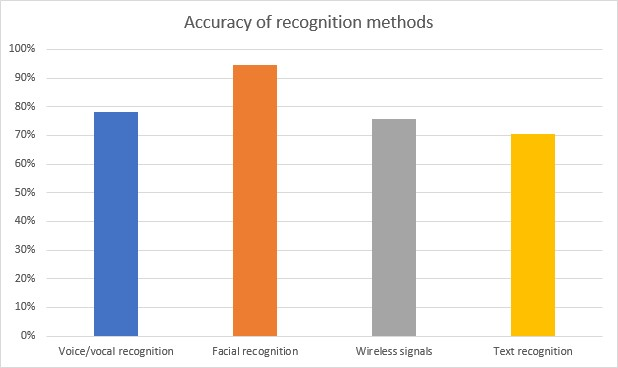
\includegraphics[width=0.45\textwidth, scale=1]{emotion_recognition_accuracy.jpg}
    \caption{Accuracy of recognition methods}
\end{figure}

Besides accuracy, two more restraints are defined:
\begin{enumerate}
    \item{If at all possible, all code and libraries used must be open source.}
    \item{The prototype has to display the predicted emotions in an interactive way.}
\end{enumerate}
Due to these requirements, and our choice to use facial expression recognition, the main research question
of this paper is: \emph{Does the visualization of emotions of young people (aged 16-26) by facial expression
recognition software, lead to discussion regarding the displayed content?}

By working towards answering this question, we are developing a prototype that collects the relevant information
that is required for the goal of the project: starting a meaningful conversation between young adults, regarding
a specific subject. Furthermore, if the prototype proves to be useful and provides valid data, it might be used in subsequent
research as a tool for collecting data.

%------------------------------------------------

\section{Related work}
Our project, as defined by the Waag Society, is already based on two previous research projects. The first
project explores a method to sympathize with other people's emotions around heritage objects. Young people,
teachers, and heritage professionals each map their emotions around a certain heritage topic and use that
mapping as a starting point for discussion \cite{emotionnetworking2017}. The goal of this research is very
similar to our own, however the means to reach that goal differ, in that our research aims to use technology
to read the emotions of the participants, as opposed to mapping them themselves.

The second project examines how participation, narratives, digital media, and atmosphere affect museum
visitors when visiting an exhibition and how exhibition makers can influence these visitor experiences.
One of the research questions is how people are emotionally affected when encountering one of
these means \cite{}. Just like the first project, our research differs due to our focus on the technological
aspect of detecting emotions.

Besides the above two project which were already defined at the start of the project, we've also found research
conducted towards facial expression recognition \cite{den2005facereader}. This research focuses solely on
detecting emotions using a camera. We also had the opportunity to try out the software created during this
research. Unlike this research, our research also seeks to visualize these predicted emotions in a meaningful
way in order to spark a discussion.

Lastly, we found a series of articles that aim to create open source facial expression recognition software
\cite{gent2016landmarks}. All of the chosen libraries and datasets were open source or easily available.
We have chosen these articles as the basis for our own prototype.

%------------------------------------------------

\section{Material}
Before creating the prototype, we were free in choosing \emph{how} we were going to implement the emotion
recognition. However, there were a couple restrictions and requirements. First, a very limited time span
to create the prototype in. The prototype had to be up and running in roughly 8 weeks so that we could
use it to perform our research. Secondly, preferable everything about the prototype had to be open source, as
requested by the Waag Society. Because of prior desk-research, combined with the above requirements, we
chose to use facial expression recognition using a camera as the basis for our prototype. This decision was
further solidified upon the discovery of several articles regarding open source facial expression software
using Python, OpenCV, Dlib, and Facial Landmarks \cite{gent2016landmarks}.

Aside from the facial expression recognition part of the project, the prototype had to be able to visualize the
emotions to allow participants to reflect on their emotions and spark a discussion. The goal of the
visualization is to show the user of the prototype their emotions over a certain time span, and allow the user
to navigate through this time span. One of our clients, the Waag Society, had already done work regarding
this subject, including the classification of emotions \cite{plutchik1980general} which we will use,
and a possible model for the visualization. We have used both the classification, as well as the model
as a basis for our prototype. The emotions we have used in our prototype are as follows: \emph{sadness,
anger, contempt, disgust, fear, happiness, neutral, and surprise}.

In order to support our user research, the prototype has to go through a number of steps. Below, each of these
steps is explained in more detail:
\begin{enumerate}
    \item{Show a video to the research subject, and start filming at the same time. Store the video for analysis.}
    \item{Once the video is done, analyze the video and store the results of the analysis.}
    \item{Visualize the generated model on-screen when the user is ready.}
\end{enumerate}

The first step, recording and storing the video, is done with OpenCV\footnote{\url{https://opencv.org}}
to allow video capture from the webcam. The prototype records at 10 frames per second (FPS).
Next, the video captures are stored locally on disk.
Displaying the video that the user of the prototype watches while he is being recorded, is considered part of
the visualization, and will be discussed later in this chapter.

The analysis and prediction of emotion from video frames is largely the same as described in the series of
articles written by Paul van Gent \cite{gent2016landmarks}. We use a trained, linear SVM machine learning model
to predict the emotions on someone's face, based on 68 specific facial landmarks. The linear SVM machine learning
model was created with scikit-learn\footnote{\url{https://scikit-learn.org}}, an open source machine learning library
for Python. In order to train the SVM model, we needed a suitable dataset of images, labeled with the
accompanying emotions. For this, we used the Cohn-Kanade and Extended Cohn-Kanade
\cite{kanade2000comprehensive, lucey2010extended} data sets.
Each image in the dataset is preprocessed before being used to train the SVM model. This includes detecting
a face on each image, cropping and resizing the face to a common size, removing all color, and using OpenCV's
CLAHE algorithm. Once the preprocessing and sorting of the images is done, we use Dlib's
\footnote{\url{https://dlib.net}} shape predictor to fetch the 68 specific facial landmarks. These landmarks,
together with the label describing the emotion on the face, are then used to train the SVM model. The total
dataset used to train the model contains 834 images. Using a larger dataset will likely result in a more accurate,
stable, result.

\begin{figure}[h]
    \centering
    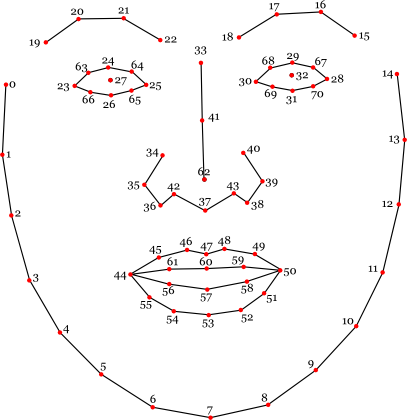
\includegraphics[width=0.45\textwidth, scale=1]{landmarks.png}
    \caption{68 facial landmarks}
\end{figure}

The recorded video from our prototype is analyzed frame by frame. Each frame goes through the same preprocessing
steps as the dataset used to train the SVM model. Once preprocessed, the 68 landmarks from each frame are then
sent through the SVM model. Since this is a probabilistic model, the percentage chance for each of the 8 emotions
is returned as a result. We found that these results could fluctuate fairly rapidly in a short number of frames.
In order to get a more stable result, we've used the average of 5 each emotion over a span of 5 frames (half a
second). This means that our final prototype predicts the emotions for every half a second of recorded video.
Once the predictions are made for the entire video, the results are stored in an Sqlite database to be used
later for the visualization. This also allows us to store the results for analysis later in our research.

\begin{figure}[h]
    \centering
    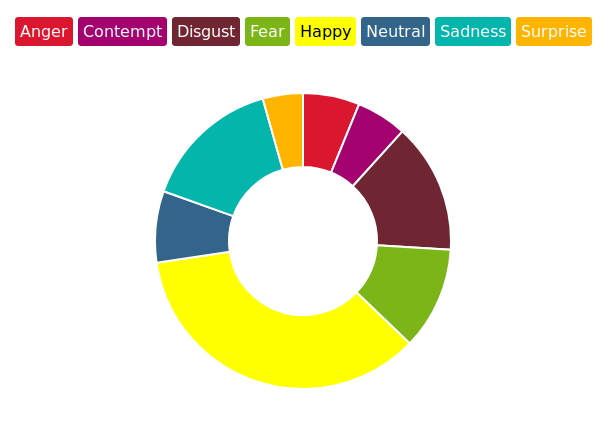
\includegraphics[width=0.45\textwidth, scale=1]{visualization.png}
    \caption{Visualized model as generated by the prototype}
\end{figure}

The visualization itself is a web application. A Flask\footnote{\url{http://flask.pocoo.org}} webserver
is used to allow API access to the rest of the prototype. HTML, CSS and Javascript are then used to
create the user interface for the prototype, including the visualization of the model.
Initially, we wanted to use Qt\footnote{\url{https://qt.io}}, a C++ UI library, but due to a lack of time and
expertise on our side, we decided to opt for something more familiar, which in this case resulted in a web
application. The user interface consists of four pages. One to display the video (and start the recording),
one to manage the sessions with our research participants, one to create a new session, and lastly, one to
show the visualization. The visualization page uses doughnut charts for each recorded participants. The charts
are generated using Chart.js\footnote{\url{http://chartjs.org}}, a Javascript library for creating a multitude
of charts. The predicted emotions are displayed half a second at a time, with a time line slider to allow the
participant to scroll through the predictions throughout the video.

%------------------------------------------------

\section{Method} \label{method}
After thoroughly testing the prototype on every aspect, working towards answering the main question was imminent.
\emph{Does the visualization of emotions of young people (aged 16-26) by facial expression
recognition software, lead to discussion regarding the displayed content?}

The research that we performed was qualitative research. Our prototype was built for testing purposes, and not
as an end-product. Therefore, we greatly value any feedback and improvement suggestions for our prototype from
our research participants, as this can be used in future development. Because we are researching
different emotional reactions of users, we're looking for very specific results. This means that our research
design is very specific as well. The research design has the following requirements:
\begin{itemize}
    \item{Users of the prototype have to be in a closed-off room to prevent any distractions which can affect
    test results.}
    \item{Users of the prototype will not be given any information regarding the purpose or operation of the
    prototype, since this can affect their emotional reactions and therefore the test results.}
    \item{Users will be asked to use the prototype one-by-one.}
    \item{Users of the prototype will be asked a set of questions which will be focused on accuracy
    and improvement of the prototype.}
    \item{Each video shown by the prototype has a maximum length of one minute due to technical restrictions.}
\end{itemize}

\subsection{Participants}
The participants are aged between 16-26 years old, and were scouted at the Amsterdam University of Applied
Sciences. The participants were invited into a reserved, closed-off classroom, located at the Wibautstraat, where
they were able to test the prototype. Our goal was to invite at least 20 participants. Unfortunately, due to
technical difficulties and time restrictions, we've only managed to get 13 participants.

\subsection{Content}
The video had to provoke a measurable reaction from the subjects. Therefore, it is important that we show content
that is doing just that. Research conducted by the Journal of Social Psychology \cite{leary2015seemingly}
has shown that the strongest emotional reaction by people is caused by showing pictures of traumatic events.
However, we wanted our subjects to show multiple emotions, and not just the ones that are associated with
traumatic events, like \emph{fear} and \emph{disgust}. Therefore, we decided to show the subjects content
that is, in any way, provoking. We have selected three videos which have been edited to last roughly one minute:
\begin{enumerate}
    \item{Roast of Giel Beelen (Peter Pannekoek roast)}
    \item{Asian longnecks: Why does this culture consider this beauty?}
    \item{Failarmy, best fails of 2017}
\end{enumerate}

\subsection{Background information}
We want to know why the users show a specific emotion at a specific moment in the shown video. In order to
do so, we're trying to find any correlation between the user's origin and the shown emotion. Therefore,
we asked them the following set of questions before each session started:
\begin{itemize}
    \item{What's your name?}
    \item{What's your gender?}
    \item{How old are you?}
    \item{Do you live alone or with others?}
    \item{Where do you live?}
    \item{Were you also raised in this city?}
    \item{Do you have any siblings?}
    \item{What's your relationship status?}
    \item{What kind of education are you currently in?}
    \item{What kind of job do you have?}
    \item{Do you have any religious convictions?}
    \item{What are your hobbies?}
    \item{Do you often go abroad?}
    \item{Do you speak any foreign languages?}
\end{itemize}

\subsection{Recording the participants}
To give a clear impression of how the sessions were conducted, see the step-by-step description below.
\begin{enumerate}
    \item{The participant and the gamemaster gather in one room, both taking place on a chair.}
    \item{The gamemaster asks the participant if they are okay with being recorded.}
    \item{The gamemaster explains how to start the movies.}
    \item{The gamemaster leaves the room.}
    \item{The participant starts the movie by clicking on a button (spacebar).}
    \item{The video (<1 minute) starts on the laptop.}
    \item{The webcam starts recording the participant while they are watching the video.}
    \item{After the video ends, the gamemaster joins the participant again.}
    \item{The gamemaster pressed a button to show the visualized model on the laptop.}
\end{enumerate}

\subsection{Conversation with the participant}
After the sessions have been conducted, we’re looking for answers. Does the visualized model show the
correct emotions according to what the users have experienced? Does the prototype have enough incentive to start
a discussion regarding the shown content? To get answers to these questions, we've asked our participants
the following set of questions:
\begin{itemize}
    \item{What did you see in the video?}
    \item{How do you feel about it?}
    \item{Why do you feel that way?}
    \item{Take a look at the model. What do you think it shows?}
    \item{\emph{The gamemaster explains the model.} Does the model show how you felt about the video?}
    \item{How do you feel about the concept "Showing a video to provoke an emotional reaction?"}
    \item{What do you think about the prototype and the visualized model?}
    \item{Do you think this contributes to starting a conversation regarding people's emotions?}
    \item{Do you see yourself discussing your emotions with other people regarding the shown content?}
\end{itemize}


%------------------------------------------------

\section{Results} \label{results}
As described in section \ref{method}, we have conducted prototype testing sessions with 13 participants.
For each of these participants, we have two pieces of data:
\begin{itemize}
    \item{Predicted emotions during the shown video, created by the prototype}
    \item{Results from the interview we had with each participant during the testing}
\end{itemize}
Furthermore, for every of the three available videos, we have expectations regarding the emotions at certain
times of the video. Using these pieces of data, we are interested in the following information from analyzing
the results:
\begin{enumerate}
    \item{Do the participants agree with the emotions predicted by the prototype?}
    \item{Do the predicted emotions coincide with the expectations we had for certain videos?}
\end{enumerate}
The first questions can be answered by cross-checking the data that the prototype generated, against the
answers from the participants during the interview. The second question can be verified by checking the
expected emotions at certain times in a video, against the average of all the participants who watched that
video. This will make it clear whether the expected emotion is also the dominant emotion at that time.
Finally, we can combine questions 1 and 2. If both results are positive; that is, the predicted emotions by the
prototype match up with our expectations, and are valid according to the participant, then we can conclude
that it's highly likely to be accurate.

\subsection{Test results}
We present an overview of the interview results, including demographic, as well as opinions regarding the
prototype. Furthermore, several line charts are given which show
the average emotions of all participants from each video, and the expected emotions as a dashed vertical line.

The analyzing of the data generated by the prototype was done using some custom code. This analyzer tool was
created using Python and the matplotlib\footnote{\url{https://matplotlib.org}} library to generate the charts.
The analysis tool is available as well: \url{https://github.com/drtheuns/minor_riet_analysis}

\subsection{Interview results}
The interview contained several questions consisting questions about the background of the participant and
questions about the experience regarding the prototype.

The total number of participants was 13. The genders of the participants contained 11 men and 2 women.
The participants differed in age, 9 participants were aged between 20-23, 3 participants between 24-27 and 1
of the participants was aged 28-30. Only one of the participants was an only child, all the other participants
had a family composition which contained one or more brothers or one or more sisters. 9 out of 13
participants didn't have a religious conviction, 2 are Atheists, 1 is Islam and the last one doesn't believe
in anything. 11 out of 13 of the participants live in Noord-Holland, the two other provinces are Flevoland and
Zuid-Holland. Also 11 out of 13 participants live in a city, the two others live in a village. 7 out of 13
participants live with their parents, 5 live on their own and 1 participant lives together with their partner.
8 out of the 13 participants are in a relationship, 4 are single and 1 participant is engaged.
Of the respondents, 11 out of 13 follow a higher professional education, the other two study at university level.
The disciplines consist largely (10/13) of ‘Exact and Informatics’ in addition to ‘Behavior and Society’,
‘Education and Upbringing’ and ‘Law and Administration’. 10 participants are in the last (fourth) year of their
education, two of them are in their third year and one of them in the second year of their education.
12 out of 13 participants have a job besides their study. 8 people did come in contact with foreign religions.

The questions from the interview have validated that 12 of the 13 participants found the visualized model clear
and understood what the model showed. Of these participants 11 of the 13 indicated that the emotions that the
model showed corresponded to the emotions that they felt during the video. 8 Participants indicated that they
showed the emotion happy, in all of these cases the visualized model corresponded with this emotion.
With the emotion ‘disgust’ there is 1 person who has indicated to have actually experienced this emotion,
yet the model showed differently and 6 of the 13 people showed the emotion disgust at some point or time frame
in the video.

The interview showed that everyone partially understood the visualized model, but that they did not immediately
see that the model showed the emotions over time. On the other hand, all participants were enthusiastic about
the overall visualized model after they had been given an explanation of how the visualized model worked
exactly. 12 of the 13 participants also found it interesting to see their own emotions; in addition,
the same 12 people felt that the prototype can certainly contribute to stimulating a discussion.
The participants indicated there must be a certain form of intelligence or an age, older people will not be
able to fully understand this prototype and thus ultimately not achieve the goal.

\subsection{Expected emotions}
For each video we had a number of expectations. These differ from general expectation (e.g. a video will be
mostly neutral), or very specific expectations (e.g. at 9 seconds in video "Failarmy" we expect happiness).
Here we enumerate and explain our expectations.

For the first video, \emph{Failarmy}, we expected 5 different moments where the research participant watching
the video would laugh. The reason for this being that this video consists of short humorous clips. These 5
moments are points in the video with climaxes to the clips. Laughter translates to happiness in our prototype,
therefore, there are 5 moments where we expect to see happiness in the charts. As mentioned above,
these are visible in figure \ref{chart_failarmy} as the dashed vertical lines.

For the second video, \emph{Neck}, we expected the majority of the video to be a mix between neutral and disgust.
We expect these emotions in particular because we expect people to not be deeply touched by the beauty
traditions of other cultures. Disgust, in particular, we expect due to not understanding or acknowledging the
culture depicted in the video as valid. Throughout the video, there are two moments in particular where we
expect a spike of disgust. The first is between 23 and 25 seconds. At this moment in the video, a child is first
shown wearing the neck coils. This, combined with the narrator mentioning that adding and maintaining these coils
is "a painful process", cause us to believe that there will be a spike in disgust. Similarly, we expect another
spike between 46 and 49 seconds, due to very comparable reasons; the video shows more coils being added to a
child, and the narrator mentions that "pain is a requirement". These two areas are marked on figure
\ref{chart_neck} as blue colored areas.

For the last video, \emph{Roast}, we expected 6 different points of laughter -- happiness -- throughout
the video. As this was another comedy video, the expected points were moments in which a joke had just been told.
Much like \emph{Failarmy}, these points can be seen on figure \ref{chart_roast} as vertical lines.

\begin{figure}[H]
    \centering
    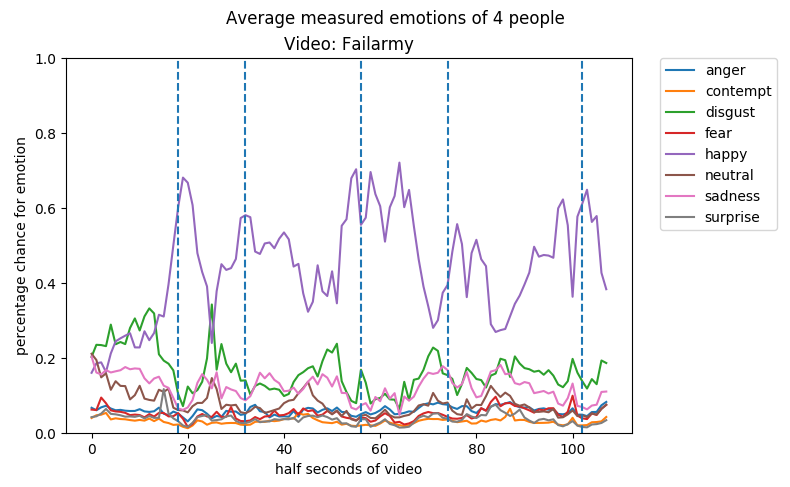
\includegraphics[width=0.5\textwidth, scale=1]{chart_failarmy_small.png}
    \caption{Average emotions of participants with video "Failarmy"}
    \label{chart_failarmy}
\end{figure}

\begin{figure}[H]
    \centering
    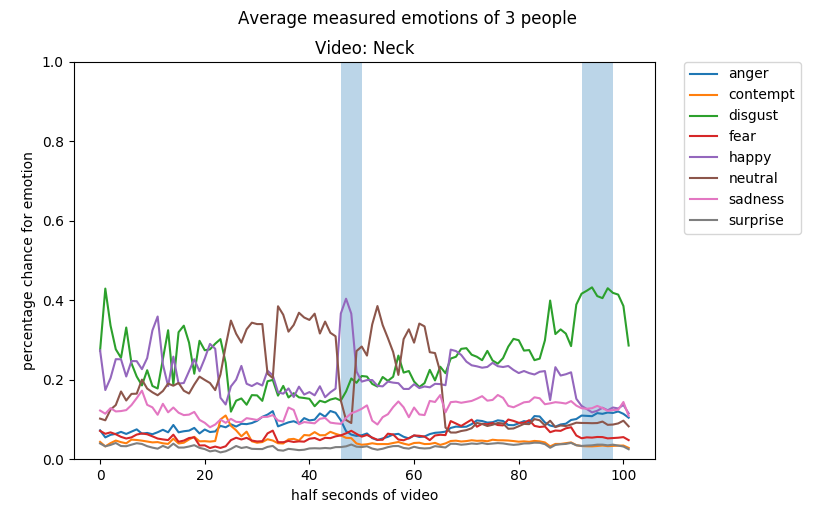
\includegraphics[width=0.5\textwidth, scale=1]{chart_neck_small.png}
    \caption{Average emotions of participants with video "Neck"}
    \label{chart_neck}
\end{figure}

\begin{figure}[H]
    \centering
    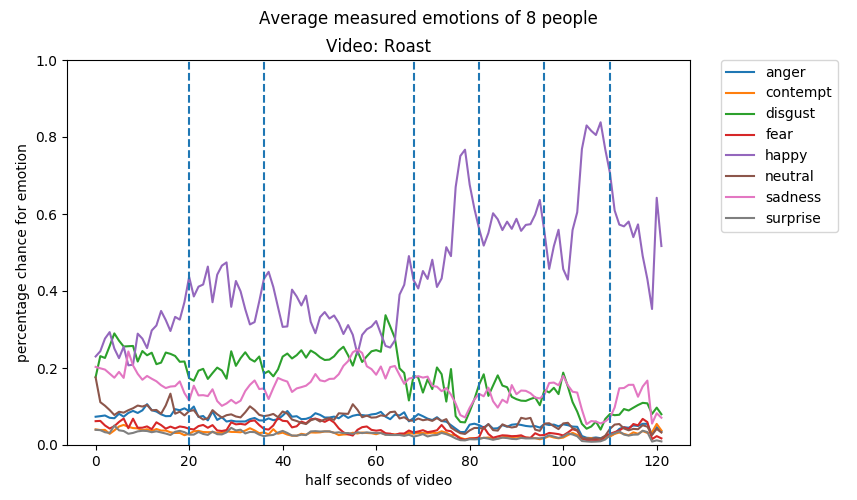
\includegraphics[width=0.5\textwidth, scale=1]{chart_roast_small.png}
    \caption{Average emotions of participants with video "Roast"}
    \label{chart_roast}
\end{figure}

Based on the above charts regarding the measured emotions versus the expected emotions, in most cases the
expectations seems to have come true. In figure \ref{chart_neck}, however, the expectation of disgust between
23 and 25 seconds seems to have been wrong, as happiness seems to be the most dominant emotion. Towards the end
of \emph{Neck}, there is also an increase in chance for happiness, alongside disgust.

Another interesting moment can be seen in figure \ref{chart_failarmy} around 12.5 seconds into the video (x=25).
Disgust takes over for a short moment in between two moments where happiness had been the emotion with the
highest percent chance.

%------------------------------------------------

\section{Discussion}
In section \ref{results} we defined two questions that, when answered, can give a more conclusive image of the
results. Here we will explore our interpretation of the data and answer these questions.

Our first question was: \emph{Do the participants agree with the emotions predicted by the prototype?}.
Out of the 13 research participants, 12 agreed that the emotions depicted by the prototype, were correct with
how they felt. Therefore, we can conclude that yes, the participants mostly agreed with the results from the
prototype. One emotion often stood out as possibly wrong, namely \emph{disgust}. Many people also agreed,
however, that this might be because of they way they look normally. This could mean that either people often
look with disgust by default, or that neutral and disgust were not properly distinguished from each other by
the prototype. This could be solved by either letting the participants review the video of themselves to see
if they agree with the judgment of the prototype, or by improving the dataset used to train the SVM model,
thereby increasing the accuracy.

Our second question, \emph{Do the predicted emotions coincide with the expectations we had for certain videos?},
can largely be answered by looking at the charts. Here we can see that in most cases, the expectations and
predicted emotions by the prototype match. Only in 1 instance was the expected emotion wrong from the measured
emotions. This was the expectation of disgust around 23 to 25 seconds in the \emph{Neck} video. One possible
explanation for this discrepancy could be the small amount of people that have watched the video (3 people).
It is possible that a single participant skewed the results because they attribute for a third of the average.
In all cases, however, the relatively small number of participants could mean that there is not enough data to
give a conclusive answer.

If we combine the positive answers for both of the above questions, we get a fairly clear image of the accuracy
and usability of the prototype. Although further improvements are necessary, for example a larger dataset,
the prototype works sufficiently well to be used in starting a discussion. Out of 13 participants, 12 agreed that
the visualization, especially in group settings, is capable of helping in starting a discussion regarding their
emotions on a specific subject.

%------------------------------------------------

\section{Conclusion}
Research question
What have we done / defined
User research
Conclusion on the prototype
Some tips for subsequent research

At the beginning of this research we paper, we defined a research question to be answered. This question was:
\emph{Does the visualization of emotions of young people (aged 16-26) by facial expression recognition software,
lead to discussion regarding the displayed content?}. In order to answer this question, we first defined how
we were going to capture emotions using technology. Once we reduced the scope to facial expression recognition,
we could continue with deciding how to visualize these captured emotions. We defined the emotions to
\emph{sadness, anger, contempt, disgust, fear, happiness, neutral, and surprise}, and chose a doughnut chart
as model for the visualization, based on prior research by the Waag Society. We then created a prototype
using open source tools and libraries, capable of predicting emotions from video and visualizing them according
to the aforementioned model.
Finally, we used the created prototype to conduct our user research. We tested the prototype with 13 different
subjects while interviewing them. The subsequent data analysis concluded that the prototype works largely as
expected. Our expectations and the results from the prototype were mostly correct, and X out of the 13 subjects
agreed with the emotions recognized by the prototype. The user research and data analysis also showed us the
imperfections of the prototype. This includes a number of unexpected emotions measured by the prototype.
This could be explained by too small of a dataset used to train the machine learning model responsible for
predicting the emotions. This is, however, something that would have to be researched in more detail in further
research.
We recommend further studies to focus on improving the visualization according to the feedback given to us by
our research subjects. Furthermore, increasing the dataset for the machine learning, and performing the user
research on a larger group of subjects. Additionally, the stability and speed of the prototype could also be
significantly improved, perhaps by switching over from Python to C++, and processing the video while it is still
being recorded.

%------------------------------------------------

\section{Acknowledgment}
This research was supported by the Amsterdam University of Applied Sciences, the Waag Society research
institute, and Research Group Crossmedia. We thank Bernadette Schrandt for all the assistance
with the research, including guidance and feedback. We thank Lodewijk Loos and Douwe-Sjoerd Boschman
from Waag Society for the assistance during the creation of the prototype. We thank Wouter Meys for setting
up the minor and advice with the research. Lastly, we would like to thank all the participants who helped
us test our final prototype.

%----------------------------------------------------------------------------------------
%	REFERENCE LIST
%----------------------------------------------------------------------------------------

\bibliographystyle{ACM-Reference-Format}
\bibliography{paper}

%----------------------------------------------------------------------------------------

\end{document}
